\chapter{Diversity Management for BFT Systems} 
\label{chap:lazarus_design}

This chapter presents the design of a control plane, named \system, to manage the diversity in \gls{bft} services.
The design improves the work presented in the previous chapter with new data and clustering techniques, introduces a new metric to evaluate vulnerabilities severity, and propose a strategy to minimize the risk of having common failure modes in replicated systems.
In the end, we validate this proposal against other strategies.

\note{We need to clarify that \system is proactive and \sieveq is reactive, they can be used together. E.g., when there is a problem the controller increases the risk}
\note{patches:Patches take time to apply~\cite{Frei:2010}
MAking exploit from patches that were not yet released!!!\cite{Brumley:2008}
THE NEED FOR AUTOMATIC PATCHING~\cite{Nappa:2015} --shared code, one takes the patch and the other no}

\section{Overview}
\system is a control plane solution that automatically changes the attack surface of a \gls{bft} system in a dependable way.
\system continuously collects security data from \gls{osint} feeds on the internet to build a knowledge base about the possible vulnerabilities, exploits, and patches related to the systems of interest.
This data is used to create clusters of similar vulnerabilities, which potentially can be affected by (variations of) the same exploit.
These clusters and other collected attributes are used to analyze the risk of the \gls{bft} system becoming compromised due to common vulnerabilities.
Once the risk increases, the control plane replaces a potentially vulnerable replica by another one, trying to maximize the failure independence of the replicated service.
Then, the replaced node is put on quarantine and updated with the available patches, to be re-used later.


%In summary, we make the following contributions: 

%\begin{enumerate}

%\item A method for assessing the risk of a group of replicas being compromised based on the security news feeds available on the internet. 
%The method overcomes limitations from works that use the \gls{nvd} data for managing the replicas vulnerability independence (Section~\ref{sec:metric});

%\item An evaluation of our risk management method based on real historical vulnerability data showing its effectiveness in keeping a group of replicas safe from common vulnerabilities (Section~\ref{sec:diversity});

%\end{enumerate}


In a nutshell, as displayed in~Figure~\ref{fig:overview}, \system provides a distributed operating system for \gls{bft}-replicated services.
The system manages a set of nodes that run \emph{unmodified replicas} (encapsulated in \glspl{vm} or containers) in its execution plane. 
Each node must have a small \gls{ltu} that allows the activation and deactivation of replicas as demanded by the \system \emph{Controller}, in the control plane.
The controller decides which software should run at any given time by monitoring the vulnerabilities that potentially exist in the pool of replicas, aiming to minimize the risk of having several nodes being compromised by the same attack.

\begin{figure}[t]
\begin{center}
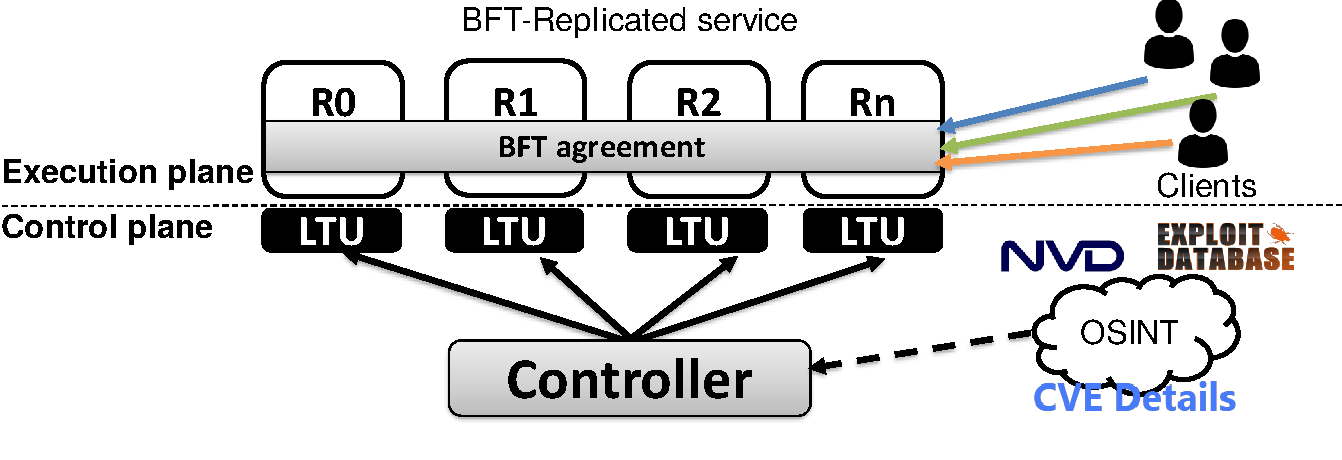
\includegraphics[width=0.8\columnwidth]{images/images/overview.pdf}
\caption{\system overview.}
\label{fig:overview}
\end{center}
\end{figure}


\section{System Model}
\label{sec:systemmodel}

\system system model shares some similarity with previous works on the proactive recovery of \gls{bft} systems~\cite{Castro:2002,Platania:2014,Sousa:2010,Roeder:2010}.
More specifically, we consider a \emph{hybrid system model} composed of two planes (see Figure~\ref{fig:overview}) with different properties and assumptions:

\begin{itemize}

\item \textbf{Execution Plane:} 
This plane is composed of replica processes that can be subject to Byzantine failures.
Therefore, a Byzantine replica can try to mislead the other replicas or the clients.
These replicas communicate through an asynchronous network that can delay, drop or modify messages, just like most \gls{bft} system models~\cite{Castro:2002,Kotla:2010,Bessani:2014,Aublin:2015}.
This plane hosts $n$ replicas from which at most $f$ can be compromised at any given moment.
We consider the typical scenario in which $n=3f+1$~\cite{Castro:2002,Kotla:2010,Moniz:2011,Bessani:2014,Aublin:2015}, but the exact resiliency bound is ortogonal to our design.

\item \textbf{Control Plane:}  
In this plane, we assume that each component can only fail by crashing. 
Each \emph{node} hosting processes contains a \gls{ltu}, and there is a logically-centralized controller to reconfigure the system, just like what has been used in several previous works on proactive recovery (e.g.,~\cite{Roeder:2010,Platania:2014,Sousa:2010}).
The failures of such components do not compromise the liveness and safety of the service as long as the control plane is recovered before $f$ replicas fail.
For simplicity, in this chapter, we address this component as a logical-centralized controller, which requires stronger assumptions. 
However, in Chapter~\ref{chap:lazarus_implementation} we introduce and discuss a \gls{bft} control plane version.


\end{itemize}

Besides the execution and control planes, we assume the existence of two types of external components: (1) clients of the replicated service, which can be subject to Byzantine failures; (2) \gls{osint} sources (e.g., \gls{nvd}, ExploitDB) that cannot be subverted and controlled by the adversary.
In practice, this assumption led us to consider only well-established and authenticated data sources.
Dealing with untrusted sources is an active area of research in the threat intelligence community (e.g.,~\cite{Sabottke:2015,Liu:2015}), which we consider out of the scope of this thesis.


%\section{Execution Plane}
%\label{sec:executionplane}

%The Execution Plane can accomodate any replicated system that already levareges on the existence of a controller node (e.g.,~\cite{Sousa:2010,Roeder:2010,Platania:2014,Garcia:2016}) or any \gls{bft} system that would benefit from the \system assistence (e.g.,~\cite{Sousa:2018}). 


%\section{Control Plane}
%\label{sec:controlplane}

%\system is the first control plane that automatically changes the attack surface of a \gls{bft} system in a dependable way.
%\system continuously collects security data from \gls{osint} feeds on the internet to build a knowledge base about the possible vulnerabilities, exploits, and patches related to the systems of interest.
%This data is used to create clusters of similar vulnerabilities, which potentially can be affected by (variations of) the same exploit.
%These clusters and other collected attributes are used to analyze the risk of the \gls{bft} system becoming compromised due to common vulnerabilities.
%Once the risk increases, \system replaces the potentially vulnerable replica by another one, trying to maximize the failure independence of the replicated service.
%Then, the replaced node is put on quarantine and updated with the available patches, to be re-used later.
%These mechanisms were implemented to be fully automated, removing the human from the loop.

%The current implementation of \system manages 17 \gls{os} versions, supporting the \gls{bft} replication of a set of representative applications.
%The replicas run in \glspl{vm}, allowing provisioning mechanisms to configure them. 
%We conducted two sets of experiments, one demonstrates that \system risk management can prevent a group of replicas from sharing vulnerabilities over time; the other, reveals the potential negative impact that virtualization and diversity can have on performance. 
%However, we also show that if naive configurations are avoided, \gls{bft} applications in diverse configurations can actually perform close to our homogeneous bare metal setup.

\section{Diversity of Replicas}
\label{sec:diversityofreplicas}

%BFT-replicated services running on \system are composed by $n$ replicas.
For our purposes, each \replica is composed of a stack of software, including an \gls{os} (kernel plus other software contained in an \gls{os} distribution), execution support (e.g., \gls{jvm}, \gls{dbms}), a \gls{bft} library, and the service that is provided by the system.
%(see Figure~\ref{fig:arch1}).
The set of $n$ replicas is called a \configuration.



The fault independence of the replicas is improved when different \gls{ots} components are employed in the software stack~\cite{Deswarte:1998}. 
For example, it has been shown that using distinct \glspl{db}~\cite{Gashi:2007}, \glspl{os}~\cite{Garcia:2013}, and filesystems~\cite{Castro:2003,Bairavasundaram:2009}, can yield important benefits in terms of fault independence. 
In addition, automatic techniques, like randomization/obfuscation of \glspl{os}~\cite{Roeder:2010} and applications~\cite{King:2016}, could enhance diversity.
Although \system can also exploit these automatic techniques, we center our attention on diverse \gls{ots} components. 
In particular, \system monitors the disclosed vulnerabilities of all elements of the replicas' software stacks to assess which of them may contain common vulnerabilities.  
As in Chapter~\ref{chap:datasource}, we focous on \gls{os} diversity here. 
Moreover, we do not explicitly consider the diversity of the \gls{bft} library (i.e., the protocol implementation) or the service code implemented on top of it.
Four facts justify this decision: (1) N-version programming is too costly for this~\cite{Avizienis:1977}; (2) there have been some works showing that such protocol implementations can be generated from formally verified specifications~\cite{Hawblitzel:2015,Rahli:2018}; (3) the relatively small size of such components (e.g., a key-value store on top of BFT-SMaRt has less than 15k lines of code~\cite{Bessani:2014}) make them relatively simple to test and assess with some confidence~\cite{Martins:2013,Lee:2014}; and (4) there are no reported vulnerabilities about these systems to support our study.
Notice that, although we do not explicitly consider the diversity of \gls{bft} libraries, nothing prevents \system from monitoring them (when several alternatives become available). 
Additionally, as a pragmatic approach, we could employ automatic diversity techniques in this layer~\cite{Platania:2014,Roeder:2010}.


\section{Diversity-aware Reconfigurations}
\label{sec:metric}

One of the main contributions of this thesis is the vulnerability evaluation method used to assess the risk of having replicas with shared vulnerabilities.
This section details this method.

\subsection{Finding Common Vulnerabilities}
\label{sec:common_vulnerabilities}

%\gls{nist}'s \gls{nvd}~\cite{nvd} is the authoritative data source for disclosure of vulnerabilities and associated information~\cite{Massacci:2010}. 
%\gls{nvd} aggregates vulnerability reports from more than 70 security companies, advisory groups, and organizations, thus being the most extensive vulnerability database on the web. 
%All data is made available as \gls{xml} data feeds, containing the reported vulnerabilities on a given period. 
%Each \gls{nvd} vulnerability receives a unique identifier and a short description provided by the \gls{cve}~\cite{cveterm}. 
%The \gls{cpe}~\cite{cpe} provides the list of products affected by the vulnerability and the date of the vulnerability publication.
%The \gls{cvss}~\cite{cvss} calculates the vulnerability severity considering several attributes, such as the attack vector, privileges required, exploitability score, and the security properties compromised by the vulnerability (i.e., integrity, confidentiality, or availability).
%WE USE THE NVD (as described in Chapter~\ref{chap:datasource}


Previous studies on diversity solely count the number of shared vulnerabilities among different \glspl{os}, assuming that less common vulnerabilities imply a smaller probability of compromising $f+1$ OSes~\cite{Garcia:2014}. 
Although this intuition may seem acceptable, in practice it underestimates the number of shared vulnerabilities due to imprecisions in the data sources. 
For example, Table~\ref{tab:missing_products} shows three vulnerabilities, affecting three different \glspl{os} at distinct dates.
At first glance, one may consider that these \glspl{os} do not share vulnerabilities.
However, a careful inspection of the descriptions shows that they are very similar.
Moreover, we checked this resemblance by searching for additional information on security websites, and we found out that CVE-2016-4428, for example, also affects Solaris~\cite{solaris_report}.

\begin{table}[!t]
\begin{center}
{\small
\begin{tabular}{| p{2.8cm} | p{10.0cm} | }\hline
\textbf{CVE (affected OS)} & \textbf{Description} \\\hline\hline
CVE-2014-0157 (Opensuse 13) & \small \gls{xss} vulnerability in the Horizon Orchestration dashboard in OpenStack Dashboard (aka Horizon) 2013.2 before 2013.2.4 and icehouse before icehouse-rc2 allows remote attackers to inject arbitrary web script or HTML via the description field of a Heat template. \\ \hline
CVE-2015-3988 (Solaris 11.2) & \small Multiple \gls{xss} vulnerabilities in OpenStack Dashboard (Horizon) 2015.1.0 allow remote authenticated users to inject arbitrary web script or HTML via the metadata to a (1) Glance image, (2) Nova flavor or (3) Host Aggregate. \\ \hline
CVE-2016-4428 (Debian 8.0) & \small \gls{xss} vulnerability in OpenStack Dashboard (Horizon) 8.0.1 and earlier and 9.0.0 through 9.0.1 allows remote authenticated users to inject arbitrary web script or HTML by injecting an AngularJS template in a dashboard form. \\ \hline
\end{tabular}
}
\caption{Similar vulnerabilities affecting different OSes.}
\label{tab:missing_products}
\end{center}
\end{table}

Even with these imperfections, \gls{nvd} is still the best data source for vulnerabilities.
Therefore, we exploit its curated data feeds to obtain the unstructured information present in the vulnerability text descriptions and use this information to find similar weaknesses.
A usual way to find similarity in unstructured data is to use clustering algorithms~\cite{Jain:2010}.
Clustering is the process of aggregating related elements into groups, named clusters, and is one of the most popular unsupervised machine learning techniques. 
We apply this technique to build clusters of similar vulnerabilities (see Section~\ref{sec:clustering} for details), even if the data feed reports that they affect different products.
For example, the vulnerabilities in Table~\ref{tab:missing_products} will be placed in the same cluster as there is some resemblance among the descriptions, and they can potentially be activated by (variations of) the same exploit.

It is worth to remark that by using clusters to find similar vulnerabilities, we conservatively increase the chances of capturing shared weaknesses contributing to the score of a pair of replicas.


\subsection{Measuring Risk}
\label{sec:measurerisk}


Once the set of common vulnerabilities is found, \system needs to assign a score to each one of these vulnerabilities based on their severity.

As presented in Chapter~\ref{chap:datasource}, each vulnerability in \gls{nvd} has associated a few \gls{cvss} severity scores and metrics (two versions are currently offered, v2~\cite{cvssv2} and v3~\cite{cvssv3}). 
The scores provide a way to unify several vulnerability attributes in a value reflecting various aspects that impact security. 
The value can also be translated into a qualitative representation to assist on the vulnerability management process. 
For example, the \gls{cvss} base score categorizes a vulnerability in a severity scale as presented in Table~\ref{tab:cvss_scale}.


\begin{table}[t]
\begin{center}
{\small
\begin{tabular}{| c | c | }\hline
\textbf{Rating} & \textbf{CVSS Score} \\\hline\hline
\texttt{NONE} & 0.0 \\
\texttt{LOW} & 0.1-3.9 \\
\texttt{MEDIUM} & 4.0-6.9 \\
\texttt{HIGH} & 7.0-8.9 \\
\texttt{CRITICAL} & 9.0-10.0 \\ \hline
\end{tabular}
}
\caption{Qualititative CVSS severity rating scale.}
\label{tab:cvss_scale}
\end{center}
\end{table}

There are some differneces between \gls{cvss} v2 and v3.
In particular, the latter introduces extra metrics that allow more granularity when assessing the vulnerability characteristics (e.g., it includes \emph{User Interaction}, specifying whether the exploitation of a given vulnerability requires human intervention).


However, \gls{cvss} has some limitations that can make it inappropriate for managing the risk associated with a replicated system:
(1)  it was shown that there is no correlation between the \gls{cvss} exploitability score and the availability of exploits in the wild for the vulnerability~\cite{Bozorgi:2010}; 
(2) \gls{cvss} does not provide information about the date when a vulnerability starts to be exploited and when the patch becomes ready; 
and (3) \gls{cvss} does not account for the vulnerability age, which means that severity remains the same over the years~\cite{Frei:2006}; therefore, a very old vulnerability can end up being considered as critical as a recent one, even though for the former there has been plenty of time to update the component and/or the defenses.  
% Nuno: tirei este ponto porque aparentemente não conseguimos soluciona-lo
%; and (4) some studies have shown that CVSS may overestimate severity~\cite{Sabottke:15}; for example, vulnerabilities with larger scores do not necessarily command higher prices at black markets~\cite{Allodi:2014}.
Additionally, both \gls{cvss} specifications support temporal metrics, i.e., Temporal Metric Group. 
However, this metric group is made to be \emph{updated} by security teams of each asset. 
Therefore, it is not provided in the \gls{nvd} feeds. 
Moreover, the specification shows that \gls{cvss} does not account for increasing the base score once there is information about existent exploits. 
For example, the score of a vulnerability with a known exploit (i.e., Exploit Code Maturity as High) has the same score as a vulnerability with no information about an exploit (i.e., Exploit Code Maturity as Not defined). 

%One of the reasons for such shortcomings is related with the fact that (both versions of) the CVSS base score is mostly static, not evolving increasing its value when exploits become widely distributed. 
%In addition, metrics belong to Temporal Metric Group (described in both CVSS specifications) are not available on NVD data feeds.

%One of the reasons why such limitations occur may be related with the fact that (both versions of) CVSS do not account for increasing the base score once there is information about an existent exploit. For example, the score of a vulnerability with a known exploit (i.e., Exploit Code Maturity as High) has the same score as a vulnerability with no information about an exploit (i.e., Exploit Code Maturity as Not defined). Additionally, these metrics belong to Temporal Metric Group (described in both CVSS specifications) which is not available on NVD data feeds.


Given these shortcomings, we propose a more refined metric that is adapted to measure the risk of a \gls{bft} system configuration having replicas with shared vulnerabilities.
The metric is mostly focused on differentiating vulnerabilities by their current \emph{potential exploitability}, aiming to surpass the limitations identified above.
In this process, (1) and (2) were addressed by using additional \gls{osint} sources that provide information about exploits and dates. 
We collect data from sources like Exploit-DB~\cite{edb} for exploits, CVE-details~\cite{cvedetails} and vendor websites to get details about the patches, such as Ubuntu Security Notices~\cite{ubuntu}, Debian Security Tracker~\cite{debian}, Solaris~\cite{solaris}, Redhat~\cite{redhat}, FreeBSD~\cite{freebsd}, and Microsoft Security Advisories and Bulletins~\cite{microsoft}. In fact, often vendor sites also give additional product versions affected by the vulnerability, thus improving the accuracy of the analysis. 
Limitation (3) is settled by decreasing the criticality of a vulnerability gradually through time.


\begin{figure}[t]
\begin{center}
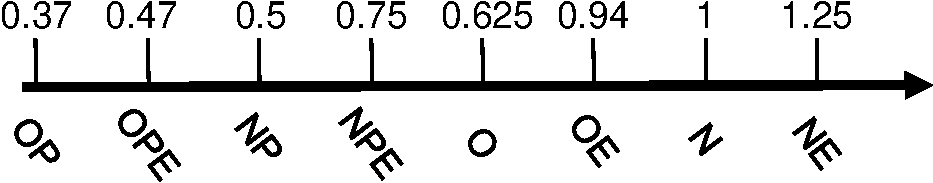
\includegraphics[width=0.7\columnwidth]{images/images/scale.pdf}
\caption{Scoring system of vulnerabilities based on age, patch, and exploit.}
\label{fig:scale}
\end{center}
\end{figure}


Our novel metric uses four factors that together contribute to the overall score. 
The starting factor is the \gls{cvss} v3 core score, as it is a reasonable basis that takes into consideration several attributes of the vulnerability.
The other three factors adjust the score taking into account the age and the availability of a patch and an exploit. 
The rationale is to rank vulnerabilities according to their possible exploitation at a given moment in time.
The resulting scale is represented in Figure~\ref{fig:scale}.
The worst scenario (higher severity score) corresponds to a vulnerability that is new (N) (i.e., recently published), for which there is an exploit already being distributed (E), and that is not yet patched -- called NE.
The best scenario (lowest score) is when a vulnerability is old (O), there is a patch (P), and apparently, no viable exploit has been crafted -- named OP. 
Between these two extremes, several cases of vulnerabilities are considered and their score calculated accordingly.

The metric is defined in Equation~\ref{eq:score}.
It is a multiplication of the \gls{cvss} v3 core score (as specified in~\cite{cvssv3}) with the three adjusting factors. 
The first is \emph{Oldness}, which causes criticality to decrease over time. 
It is harmonized by the \emph{Oldness Threshold} and the interval\footnote{\textit{Oldness Threshold} is set to 365 in our calculations; \textit{now()} and $v_i.published\_date$ return the current day and the day when the vulnerability was published, respectively.} that has passed since the vulnerability publication (Equation~\ref{eq:oldness}). 
In addition, this factor is bounded by a minimum value that impedes it from reaching zero (which would cause the vulnerability to be left unnoticed).
The second is \emph{Patched}, which reduces the severity by half when a patch is available (Equation~\ref{eq:patched}; $v_{i}.patched$ is a on/off flag).
Finally, the \emph{Exploited} factor grows severity by a quarter when an exploit is made available (Equation~\ref{eq:exploited}; $v_{i}.exploited$ is again a on/off flag).
The constants in these equations were defined to ensure the aggregated modifiers corresponds to Figure~\ref{fig:scale}.
Overall, the range of our metric is from $0.0$ to $12.5$ (similar to \gls{cvss} score $[0.0-10.0]$).



\begin{table}[h]
\begin{center}
%{\footnotesize
\begin{tabular}{ c }
%\hline

\vbox{
\begin{equation}
\begin{split}
\text{score(v$_i$)}=\text{CVSSv3(v$_i$)}\times\text{oldness(v$_i$)}\times\text{patched(v$_i$)}\times\text{exploited(v$_i$)}
\label{eq:score}
\end{split}
\end{equation}
}
%\vspace{-1mm}
\\
\vbox{
\begin{equation} 
\begin{split}
\text{oldness(v$_i$)}=\text{max}\left((1-0.25\times\frac{(\text{now()}-\text{v$_i$.published\_date)}}{\text{Oldness Threshold}}), 0.75\right)
\label{eq:oldness}
\end{split}
\end{equation}
}
%\vspace{-1mm}
\\
\vbox{
\begin{equation} 
\text{patched(v$_i$)}=0.5^{\text{v$_i$.patched}}
\label{eq:patched}
\end{equation} 
}
%\vspace{-1mm}
\\
\vbox{
\begin{equation}
\text{exploited(v$_i$)} = 1.25^{\text{v$_i$.exploited}}
\label{eq:exploited}
\end{equation}  
}
\\ 
%\hline
\end{tabular}
%}
\end{center}
\end{table}



\begin{figure}[t]
\subfloat[CVE-2018-8303.]{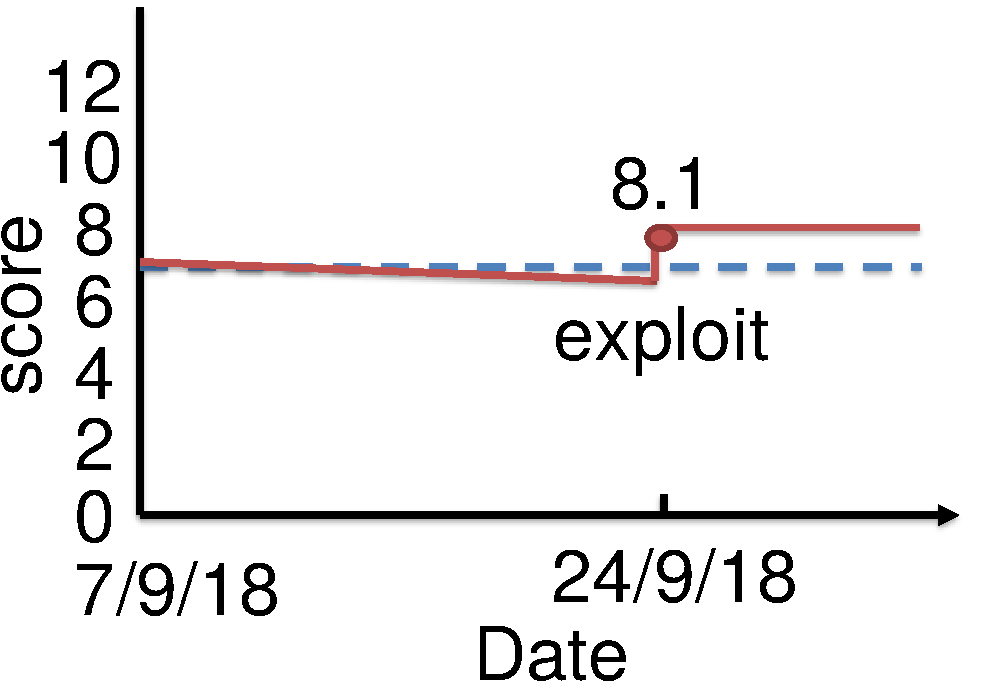
\includegraphics[width=0.34\columnwidth]{images/images/NE.pdf}\label{fig:ne}} %for Windows 10
\subfloat[CVE-2016-7180.]{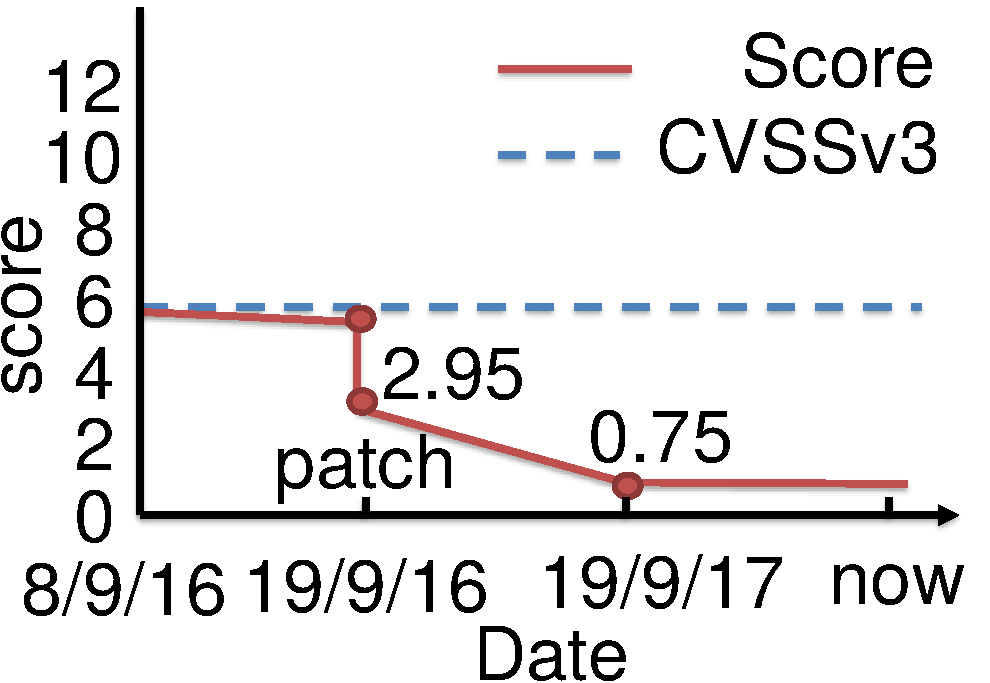
\includegraphics[width=0.34\columnwidth]{images/images/OP.pdf}\label{fig:op}}%Debian 9.0
\subfloat[CVE-2018-8012.]{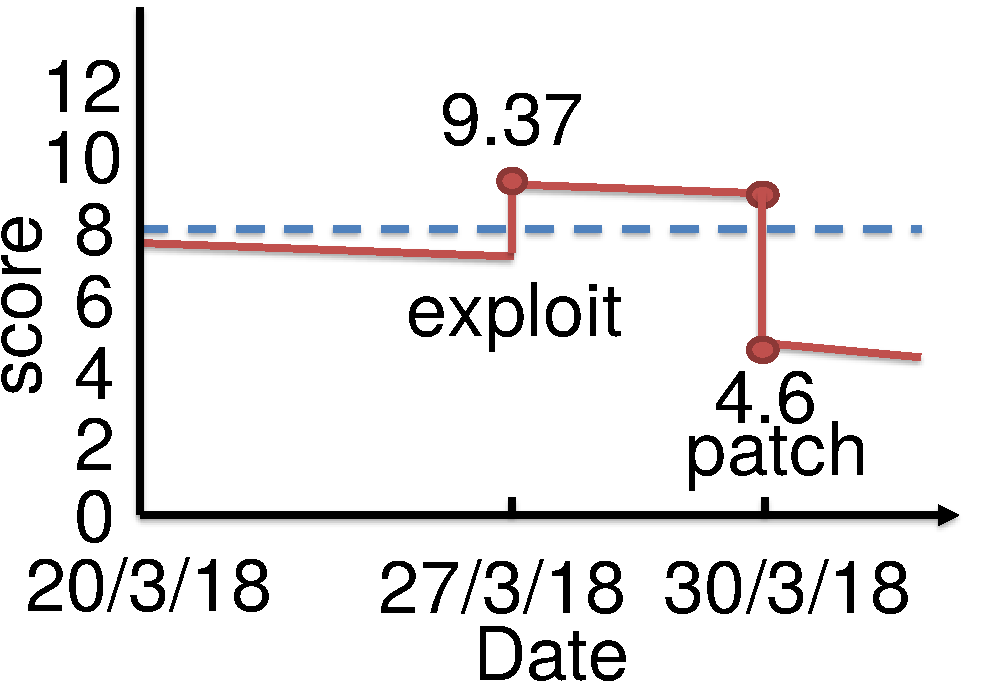
\includegraphics[width=0.34\columnwidth]{images/images/NPE.pdf}\label{fig:npe}} %Debian 9.0
\caption{Examples of \emph{score(v$_i$)} for three vulnerabilities.}
\label{fig:scoreplot}
\end{figure}


Figure~\ref{fig:scoreplot} displays our score and \gls{cvss} v3 for three example vulnerabilities. 
Case (a) corresponds to an NE, i.e., a vulnerability that is new and has no patch yet, but an exploit was made available a few days after publication. 
Our score starts by decaying slowly but then there is a jump on severity when the exploit is published.
%On the contrary, the CVSS score remains constant (approx. $6.5$).
Case (b) presents the best scenario (i.e., OP), where the vulnerability is \emph{old} and a patch was eventually distributed (and no exploit is available). Here, the severity decreases once there is a patch and over time, losing its relevance from a security perspective. 
Finally, case (c) illustrates a vulnerability that has an exploit a few days after publishing and then a patch is also created (i.e., NPE).
First, the score is raised once the exploit starts to be distributed, next it decreases three days later after the patch is released, and then continues to decay with the passage of time.


\subsection{Measuring Configurations Risk}
\label{sec:risk}

After discovering common vulnerabilities and assigning a score to them, the third step of our method is to calculate the \emph{risk of a set of replicas} to be compromised by the same vulnerability in the current threat landscape.


The risk associated with a \configuration (\ES) with $n$ replicas is given by Equation~\ref{eq:risk}. 
It sums up the score (Equation~\ref{eq:score}) of the vulnerabilities that would allow an attack to compromise simultaneously a pair of replicas $r_i,r_j \in \ES$.
%Function \emph{common()} employs our score, as it aggregates security features of a vulnerability, and other information collected from OSINT sources. To begin, the function gathers all the vulnerabilities that would allow an attack to compromise simultaneously a pair of replicas ($rc_i,rc_j$). 
More precisely, the vulnerabilities in $\mathcal{V}(r_i,r_j)$ aggregate: (i) the vulnerabilities that affect the software running in both replicas as listed in \gls{nvd} (and other \gls{osint} data); and (ii) groups of vulnerabilities that are placed in the same cluster and affect each replica in the pair. 
%The final score is normalized with function \emph{norm()} to generate a value between 0 and 1.
%Next, the function calculates the score of each vulnerability, and returns the sum of all scores. 
%The risk metric computes \emph{common()} for all combinations of replica pairs in the configuration and accumulates the values. 
%\vspace{-3mm}
%{\footnotesize

\begin{table}[h]
\begin{center}
%{\footnotesize
\begin{tabular}{ c }
%\hline

\vbox{
\begin{equation}
\mathit{risk(\ES)}=\sum_{r_i,r_j \in \ES}^{} \hspace{1.2mm} \sum_{v \in \mathcal{V}(r_i,r_j)}^{}\mathit{score(v)}
\label{eq:risk}
\end{equation}
}
\\
% \hline
\end{tabular}
%}
\end{center}
\end{table}


This metric penalizes configurations that include replica pairs containing more common weaknesses, as this is an indication that they are less fault independent.
In addition, the level of penalty is kept proportional to the severity of these vulnerabilities as observed at the time of the calculation. 
Thus, for example, replicas that share weaknesses only in the distant past are considered less risky to run in a configuration than replicas that together had recently highly exploitable vulnerabilities.

\subsection{Selecting Configurations}
\label{sec:configurations}

The last step of our method is to periodically assess the risk of a deployed configuration and its future replacement of replicas according to the evaluation of the metric of the previous section.

The bootstrap of the monitoring algorithm is simple. 
The first replica is selected randomly from the available candidates (\RS).
Then, it selects the next $n$ elements by minimizing the risk of the \ES in construction (using Equation~\ref{eq:risk}).
After the initialization, the \ES is periodically monitored and reconfigured if needed, as detailed in Algorithm \ref{alg:algorithm2}.
This is done by periodically evaluating the risk of the current \ES. 
If the risk exceeds a predefined \emph{threshold}, a mechanism is triggered to replace replicas and reduce the overall risk.
When this happens, the algorithm will pick a new replica from \RS to join \ES. 
In addition, it removes the replica that will reduce the risk.
The removed replica is set aside in a special group (\QS) to impede re-selection.
While in \QS, the replicas wait for patches before they re-join \RS and be ready to be chosen again.
Additionally, the algorithm ensures that all replicas that are running will eventually be replaced, despite their overall score.
Otherwise, the algorithm favors configurations that have lower scores by keeping them online for longer periods, allowing an attacker to gain time to discover new vulnerabilities.
To avoid this problem, the algorithm looks for the unpatched vulnerabilities with higher score affecting singles replicas.
This approach is conservative in the sense that it penalizes replicas expecting that such vulnerabilities can be unknown as common to other replicas.

\begin{algorithm}[t]
%\begin{multicols}{2}
%\SetInd{0.3em}{0.2em}
\caption{Replica Set Reconfiguration}\label{alg:algorithm2}
{\scriptsize
\ES: set replicas in the \configuration \;
$n$: number of replicas in \ES\;
\RS: set with the available replicas (not in use)\;
\QS: set of quarantine replicas\;
\BlankLine
\Fn{Monitor()}{
	\If{\Risk{\ES} $\geq$ threshold}{	
		\texttt{cadidates\_list} $\leftarrow$ $\perp$\;
		\COMBS = ${n\choose n-1}$\ES\;
		\ForEach{$ r $ in \RS}{
			\ForEach{$ \COMB $ in \COMBS}{
				\ES' $\leftarrow$ \COMB $\cup$ \{r\}\;
				\texttt{score} $\leftarrow$ \Risk{\ES'}\;
				\texttt{cadidates\_list}.add($\langle$\ES', \texttt{score}$\rangle$)\;
			}
		}
	\SC $\leftarrow$ \Rand{\texttt{cadidates\_list}} \;
	\Replace{\SC}\;		
	}
    \Else{
		\toRemove $\leftarrow$ $\perp$\;
		\texttt{maxScore} $\leftarrow$ \texttt{HIGH}\;
		\ForEach{$ r $ in \ES}{
			\texttt{avgScore} $\leftarrow$ \oldestVulnerability{r}\;
			\If{ avgScore $\geq$ maxScore}{	
				\toRemove $\leftarrow$ $r$\;
				\texttt{maxScore} $\leftarrow$ avgScore\;
			}
	}
		\If{ \toRemove $\neq$ $\perp$}{
			\texttt{cadidates\_list} $\leftarrow$ $\perp$\;				
			\ForEach{$ r' $ in \RS}{
				\ES' $\leftarrow$ (\ES $\setminus$ \{toRemove\}) $\cup$ \{r'\}\;
				%\ES' $\leftarrow$ \ES' $\cup$ \{r'\}\;
				\texttt{score} $\leftarrow$ \Risk{\ES'}\;	
				\texttt{cadidates\_list}.add($\langle$\ES', \texttt{score}$\rangle$) \;
			}
			\SC $\leftarrow$ \Rand{\texttt{cadidates\_list}} \;
			\Replace{\SC}\;
		}
	}
	\ForEach{$ r $ in \QS}{	
		\If{\patched{r} = TRUE}{	
			\QS $\leftarrow$ \QS $\setminus$ $\{r\}$\;
			\RS $\leftarrow$ \RS $\cup$ $\{r\}$\;
		}
	}
}
\Fn{updateSets(\SC)}{
		\toRemove $\leftarrow$ $x \in (\ES \setminus \SC)$\;
		\toJoin $\leftarrow$ $y \in (\SC \setminus \ES)$\;
		\QS $\leftarrow$ \QS $\cup$ $\{toRemove\}$\;
		\ES $\leftarrow$ (\ES $\setminus$ $\{toRemove\}$) $\cup$ $\{toJoin\}$\;

}
}
%\end{multicols}
\end{algorithm}


Function \emph{Monitor()} (line 5) is called on each monitoring round (e.g., at midnight every day) to evaluate the configuration that is executing.
%Consider a \ES that is already running with a risk$=\alpha$.
If the risk of \ES is greater or equal than a certain \emph{threshold} (line 6), the algorithm will assess which replica should be replaced.
The first step is to initialize two variables, the candidates list (line 7) and all possible combinations of $n-1$ out of $n$ elements of \ES (line 8).
Then, each element \texttt{r} in \RS (line 9) is tested as a potential substitute, i.e., as the $n^{th}$ element that would complete each of the combinations \COMB with $n-1$ replicas (line 10).
Next, we define a \ES' as the union of \COMB and $r$ (line 11).
The risk of \ES' is calculated (line 12) and added to a list that stores the tuple $\langle$\ES', \texttt{score}$\rangle$ (line 13). 
At the end of the these nested loops, we have a list with all the possible combinations of \ES and \RS together with their risk.
Then, the function \Rand selects a configuration randomly from the list of candidates (line 14). 
Although it is not present in the algorithm, it only selects configurations which are below the \emph{threshold} score. 
Then the algorithm updates all the sets (line 15) using the function \Replace (lines 36-40). 
To decide which element needs to be removed from \ES it makes the difference between the current \ES and \SC (line 37) and the contrary to select the element to join the \ES (line 38).
Then, \toRemove is added to \QS (line 39), removed from \ES, and the new element is added to the \ES (line 40).
 

If the risk of \ES is smaller than the \emph{threshold} (line 16) we need to assess if the \ES needs a reconfiguration.
In this scenario, we start by initializing the variable \toRemove as empty (line 17) and \texttt{maxScore} with the value of the \gls{cvss} score rating \texttt{HIGH} (line 18).
For each element of \ES (line 19) the algorithm calculates the average score of the vulnerabilities affecting \r using Equation~\ref{eq:score} (line 20).
Then, if the average vulnerability score is equals or greater than \texttt{HIGH} (or \texttt{CRITICAL}) (line 21), the variable \toRemove is set to the element \r (line 22) and the value of \texttt{maxScore} with the \texttt{avgScore} (line 23).
At the end of the loop, the algorithm knows which is the element \r from \ES that has vulnerabilities with a highest average score.
If \toRemove is empty then algorithm proceeds to line 32. 
Otherwise, the algorithm will select a new replica (line 24).
First, the \texttt{candidate\_list} is set as empty (line 25).
Next, for each element \r' in \RS (line 26) the algorithm tests a \ES' with \r' instead of \toRemove (line 27).
Then, the score for this configuration is calculated (line 28) and together with the \ES' is stored in a list of configuration candidates (line 29).
%As already described, the function \Replace updates the elements of the sets (line 31).
In the end, one of the candidate configurations is randomly selected (lines 30-35).

Finally, the \RS and \QS sets are updated. 
Each \QS element (line 32) is checked if it is fully patched (line 33).
In the affirmative case, the element is removed from \QS and added to the \RS again (lines 34-35).


For the sake of simplicity we do not present two corner cases where a \emph{system admin} may need to intervene: if the \RS runs out of elements or \emph{rand()} cannot return a configuration that minimizes the risk of the system.
One can take at least two decisions to guarantee the availability under some risk of becoming compromised: (1) increase the \emph{threshold} or (2) reset the \RS by removing the elements from \QS with fewer unpatched vulnerabilities.
Both cases are not likely to occur, but if they happen there is not much we can make to solve as we depend on the availability of replicas in \RS and patch availability to clean \QS from time to time. 

\section{Evaluation}
\label{sec:diversity}


This section evaluates how \system performs on the selection of dependable replica configurations.
As discussed in Section~\ref{sec:diversityofreplicas}, we focus our experimental evaluation solely on the OS diversity.
In particular, we considered 21 \gls{os} versions to be deployed on four replicas with the following distributions: OpenBSD, FreeBSD, Solaris, Windows, Ubuntu, Debian, Fedora, and Redhat. 

In these experiments, we emulate live executions of the system by dividing the collected data into two periods:
(i) a \emph{learning phase} covering all vulnerability data between \emph{2014-1-1} and the beginning of the \emph{execution phase}, which is used to setup the \risk's algorithm; 
and (ii) an \emph{execution phase} period that goes from January to August of 2018. 
This last period is divided into monthly intervals (JAN-AUG) allowing for eight independent tests.
For example, to run the experiment in May the \emph{learning phase} starts on \emph{2014-1-1} and ends on \emph{2018-4-30}, then the \emph{execution phase} starts on the May $1^{st}$ until the end of the month. 

The goal is to create a knowledge base in the \emph{learning phase} that is used to assess \system' choices during each interval of the \emph{execution phase}. 
A run starts on the first day of an interval and then progresses through each day of the interval until the end. 
Every day, we check if the currently executing replica set could be compromised by an attack exploring the vulnerabilities that were published in that month. 
We take the most pessimistic approach, which is to say that we consider the system to be broken if a single vulnerability comes out affecting at least two \glspl{os} that would be executing at that time and do not have a patch for it.
%Therefore, if one of the \glspl{os} already has a patch for the tested vulnerability, it is not counted as compromised.


Four additional strategies, inspired by previous works, were defined to be compared with \system (Section~\ref{sec:configurations}):

\begin{itemize}

\item \textbf{Equal:} all the replicas use the same randomly-selected \gls{os} during the whole execution. 
This corresponds to the scenario where most past \gls{bft} systems have been implemented and evaluated (e.g.,~\cite{Kotla:2010,Aublin:2015,Behl:2015,Veronese:2013,Behl:2017,Liu:2016,Yin:2003,Amir:2011,Bessani:2014,Clement:2009b}). 
Here, compromising a replica would mean an opportunity to intrude the remaining ones.

\item \textbf{Random:} a configuration of $n$ \glspl{os} is randomly selected, and at the beginning of each day, a new \gls{os} is randomly picked to replace an existing one. 
This solution represents a system with proactive recovery and diversity, but with no informed strategy for choosing the next \configuration.

\item \textbf{Common:} This strategy is the straw man solution to prevent the existence of shared vulnerabilities among \glspl{os}. 
This strategy minimizes the number of common vulnerabilities for each set and was introduced in previous vulnerability studies~\cite{Garcia:2012}.

\item \textbf{CVSS v3:} This strategy is very similar to ours as it tries different combinations to find the best configuration that minimizes the sum of \gls{cvss} v3 score.


\end{itemize}


\subsection{Diversity vs Vulnerabilities}
We evaluate how each strategy can prevent the replicated system from being compromised. 
Each strategy is analyzed over $1000$ runs throughout the execution phase in monthly slots. 
Different runs are initiated with distinct random number generator seeds, resulting in potentially different \gls{os} selections over the time slot. 
On each day, we check if there is a vulnerability affecting more than one replica in the current \configuration, and in the affirmative case the execution is stopped.

\begin{figure}[t]
\begin{center}
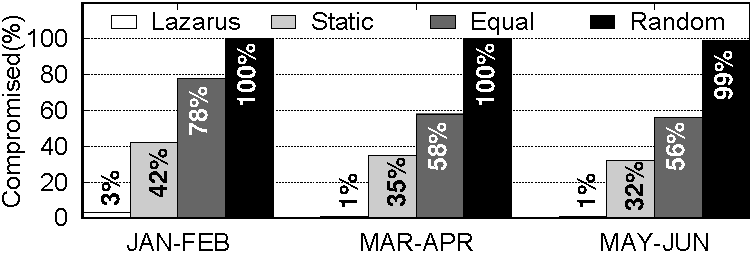
\includegraphics[width=\columnwidth]{images/gnuplot/executions/execution.pdf}
\caption{Compromised system runs over eight months.}
\label{fig:all_vulns}
\end{center}
\end{figure}


\textbf{Results:} Figure~\ref{fig:all_vulns} compares the percentage of compromised runs of all strategies. 
Each bar represents the percentage of runs that did not terminate successfully (lower is better). 
In all three periods, \system presents the best results. 
The \emph{Random} and \emph{Equal} strategies perform worse because eventually, they pick a group of OSes with common vulnerabilities as they do not make decisions with specific criteria. 
Although some criteria guide the other strategies, most of them present a majority of executions compromised during the experiments.
This result provides evidence for the claim that \system improves the dependability, reducing the probability that $f+1$ \glspl{os} eventually become compromised. 
Nevertheless, the results from May deserved a more careful inspection. 
We have identified some \glspl{cve} that make it very difficult to survive to common vulnerabilities even using the \system strategy.
For example, CVE-2018-1125, CVE-2018-8897, and CVE-2018-8897 that not only affect a few Ubuntu releases but also affect Debian releases simultaneously.
There are also a set of vulnerabilities affecting several Windows releases (e.g., CVE-2018-8134 and CVE-2018-0959). 
We also found a vulnerability (i.e., CVE-2018-1111) that affects few Fedora releases and one Redhat release that was repeatedly compromising the executions.
We have made a more careful inspection of the dispersion of vulnerabilities across these months. 
Although May is not the month with most vulnerabilities, it has on average $3.05$ \glspl{os} affected by a vulnerability, and it is the highest.
This result was already observed in our previous work (see Figure~\ref{top}, in Chapter~\ref{chap:datasource}) where the number of shared vulnerabilities decreases drastically between three affected \glspl{os} to four: almost $50$ vulnerabilities affecting three \glspl{os} and less than ten affects four \glspl{os}. 

One of the outcomes of this experiment is that, contrary to the intuition, not guided strategies will eventually create unsafe configurations.
%The most relevant result shows that contrary to intuition, changing \glspl{os} every day with no criteria will always create unsafe configurations.
Therefore, it is paramount to have selection strategies like the ones we use in \system.

\subsection{Diversity vs Attacks}


This experiment evaluates the strategies when facing notable attacks/vulnerabilities that appeared in the last year. 
Each attack potentially exploits several flaws, some of which affecting different OSes. 
The attacks were selected by searching the security news sites for high impact problems, most of them related to more than one CVE. 
As some of the CVEs include applications, we added more vulnerabilities to the database for this purpose. 
We have considered the attacks described in Table~\ref{tab:special_vulns}: 

\begin{table}[t]
{\scriptsize

\begin{tabular}{  | r  p{0.80\textwidth} | }\hline
\textbf{WannaCry}~\cite{wannacry} & \emph{On Friday, May 12, 2017, the world was alarmed to discover a widespread ransomware attack that hit organizations in more than 100 countries. Based on a vulnerability in Windows' SMB protocol (nicknamed EternalBlue), discovered by the NSA and leaked by Shadow Brokers.} \\ \hline

\textbf{StackClash}~\cite{stacklash} & \emph{In its 2017 malware forecast, SophosLabs warned that attackers would increasingly target Linux. The flaw, discovered by researchers at Qualys, is in the memory management of several operating systems and affects Linux, OpenBSD, NetBSD, FreeBSD and Solaris.}\\ \hline

\textbf{Petya}~\cite{petya} & \emph{Another month, another global ransomware attack. [...] Just as it seemed that the threat of WannaCry has dissipated, organisations around the world are finding themselves under siege from a new threat. This cyberattack first hit targets in Ukraine, including its central bank, main international airport and even the Chernobyl nuclear facility before quickly spreading around the globe, infecting organisations across Europe, North America and even Australia. A day after the incident began, at least 2,000 attacks have been recored across at least 64 countries.}\\ \hline
\end{tabular}
}

\caption{Notable attacks during 2017.}
\label{tab:special_vulns}
\end{table}


Since some of these attacks might have been prepared months before the vulnerabilities are publicly disclosed, we augmented the execution phase to the full eight months. 
Therefore, we set \emph{learning phase} to begin \emph{2014-1-1} and to end on \emph{2017-12-31}. 
The \emph{execution phase} period that starts on 2018 January and finishes on August 2018. 
As before, the strategies are executed over $1000$ runs. 


\begin{figure}[t]
\begin{center}
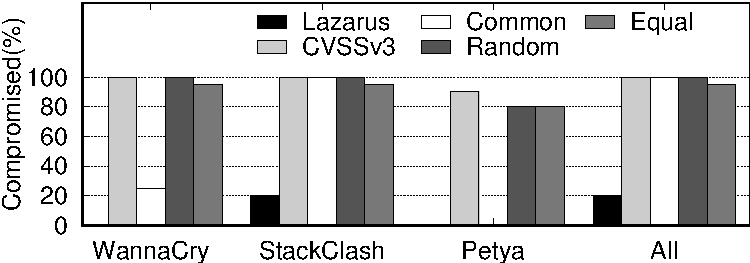
\includegraphics[width=\columnwidth]{images/gnuplot/attacks/attacks.pdf}
\caption{Compromised runs with notable attacks.}
\label{fig:special_vulns}
\end{center}
\end{figure}

\textbf{Results:}
Figure~\ref{fig:special_vulns} shows the percentage of compromised runs for each attack and all attacks put together.
\system is the best at handling the various scenarios, with almost no compromised executions.
The StackClash is the most destructive attack as it is the one affecting more \glspl{os}.
Therefore, decisions guided by criteria that aim to avoid common vulnerabilities may also fail. 
Nevertheless, the results show that such strategies do improve the resilience to attacks.



\section{Final Remarks}
\label{sec:finalremarkslazarusdesign}

\system addresses the long-standing open problem of evaluating, selecting, and managing the diversity of a \gls{bft} system to make it resilient to malicious adversaries.
This chapter shows an approach to select the best replicas to run together given the current threat landscape and evaluate the proposed strategy.
In the next chapter, we discuss how this strategy can be implemented and the overhead of using \gls{os} diversity.

